\subsection{Bezkontextové gramatiky (BG)}
Bezkontextová gramatika definuje \textbf{bezkontextový jazyk}. Je tvořena \textbf{neterminály} (proměnné), \textbf{terminály} (konstanty) a \textbf{pravidly}, které každému neterminálu definují přepisovací pravidla. Jeden neterminál označíme jako \textbf{startovní}, kde začínáme a podle pravidel je dál přepisujeme na výrazy složené z terminálu a neterminálu. Jakmile už není co přepisovat, výraz obsahuje už jen neterminály, získali jsme \textbf{slovo}.

\begin{itemize}
\item Je \textbf{uzavřená} vůči operacím \textbf{sjednocení}, \textbf{zřetězení}, \textbf{iteraci} a \textbf{zrcadlový obraz}.
\item Ke každé bezkontextové gramatice existuje \textbf{ekvivalentní zásobníkový automat}.
\end{itemize}

\subsubsection{Formální definice BG}
Bezkontextová gramatika je definována jako uspořádaná čtveřice $G = (\Pi, \Sigma, S, P)$, kde:
\begin{itemize}
	\item $\Pi$ (\textit{velké pí}) je konečná množina \textbf{neterminálních} symbolů (neterminálů).
	\item $\Sigma$ je konečná množina \textbf{terminálních} symbolů (terminálů), $\Pi \cap \Sigma = \emptyset$.
	\item $S$ je \textbf{počáteční neterminál}, $S \in \Sigma$.
	\item $P$ je konečná množina \textbf{přepisovacích pravidel}, $P \subseteq \Pi \times (\Pi \cup \Sigma)^*$.
\end{itemize}

\subsubsection{Základní pojmy}
\begin{itemize}
\item \textbf{Bezkontextový jazyk} -- formální jazyk, který je akceptovaný nějakým zásobníkovým automatem.
\item \textbf{Derivace slova} -- jedno konkrétní odvození slova pomocí gramatiky, tedy záznam postupných přepisů od startovního neterminálu po konečné slovo. Derivace se podle postupu při přepisování dělí na:
\begin{itemize}
\item \textbf{levou} -- přepisujeme nejprve levé neterminály,
\item \textbf{pravou} -- přepisujeme nejprve pravé neterminály.
\end{itemize}
\item \textbf{Derivačni strom} -- grafické znázornění derivace slova stromem. Pro všechny možné derivace (levou, pravou, moji) by měl derivační strom být \textbf{stejný}. Není-li tomu tak jedná se o \textbf{nejednoznačnou gramatiku}, což je nežádoucí jev. 
\begin{itemize}
	\item \textbf{Špatně} = A $\rightarrow$ A | $\epsilon$ (lze generovat až N způsoby), \textbf{Správně} = A $\rightarrow \epsilon$ 
\end{itemize}
\item \textbf{Chomského normální forma} -- gramatika může obsahovat pouze pravidla typu: \textbf{A $\rightarrow$ BC} nebo \textbf{A $\rightarrow$ a} nebo \textbf{S $\rightarrow \epsilon$} (pokud gramatika generuje pouze prázdný řetězec).
\item \textbf{Nevypouštějící gramatika} -- neobsahuje $\epsilon$ (\textit{epsilon}) přechody.
\end{itemize}

\begin{figure}[H]
	\centering
	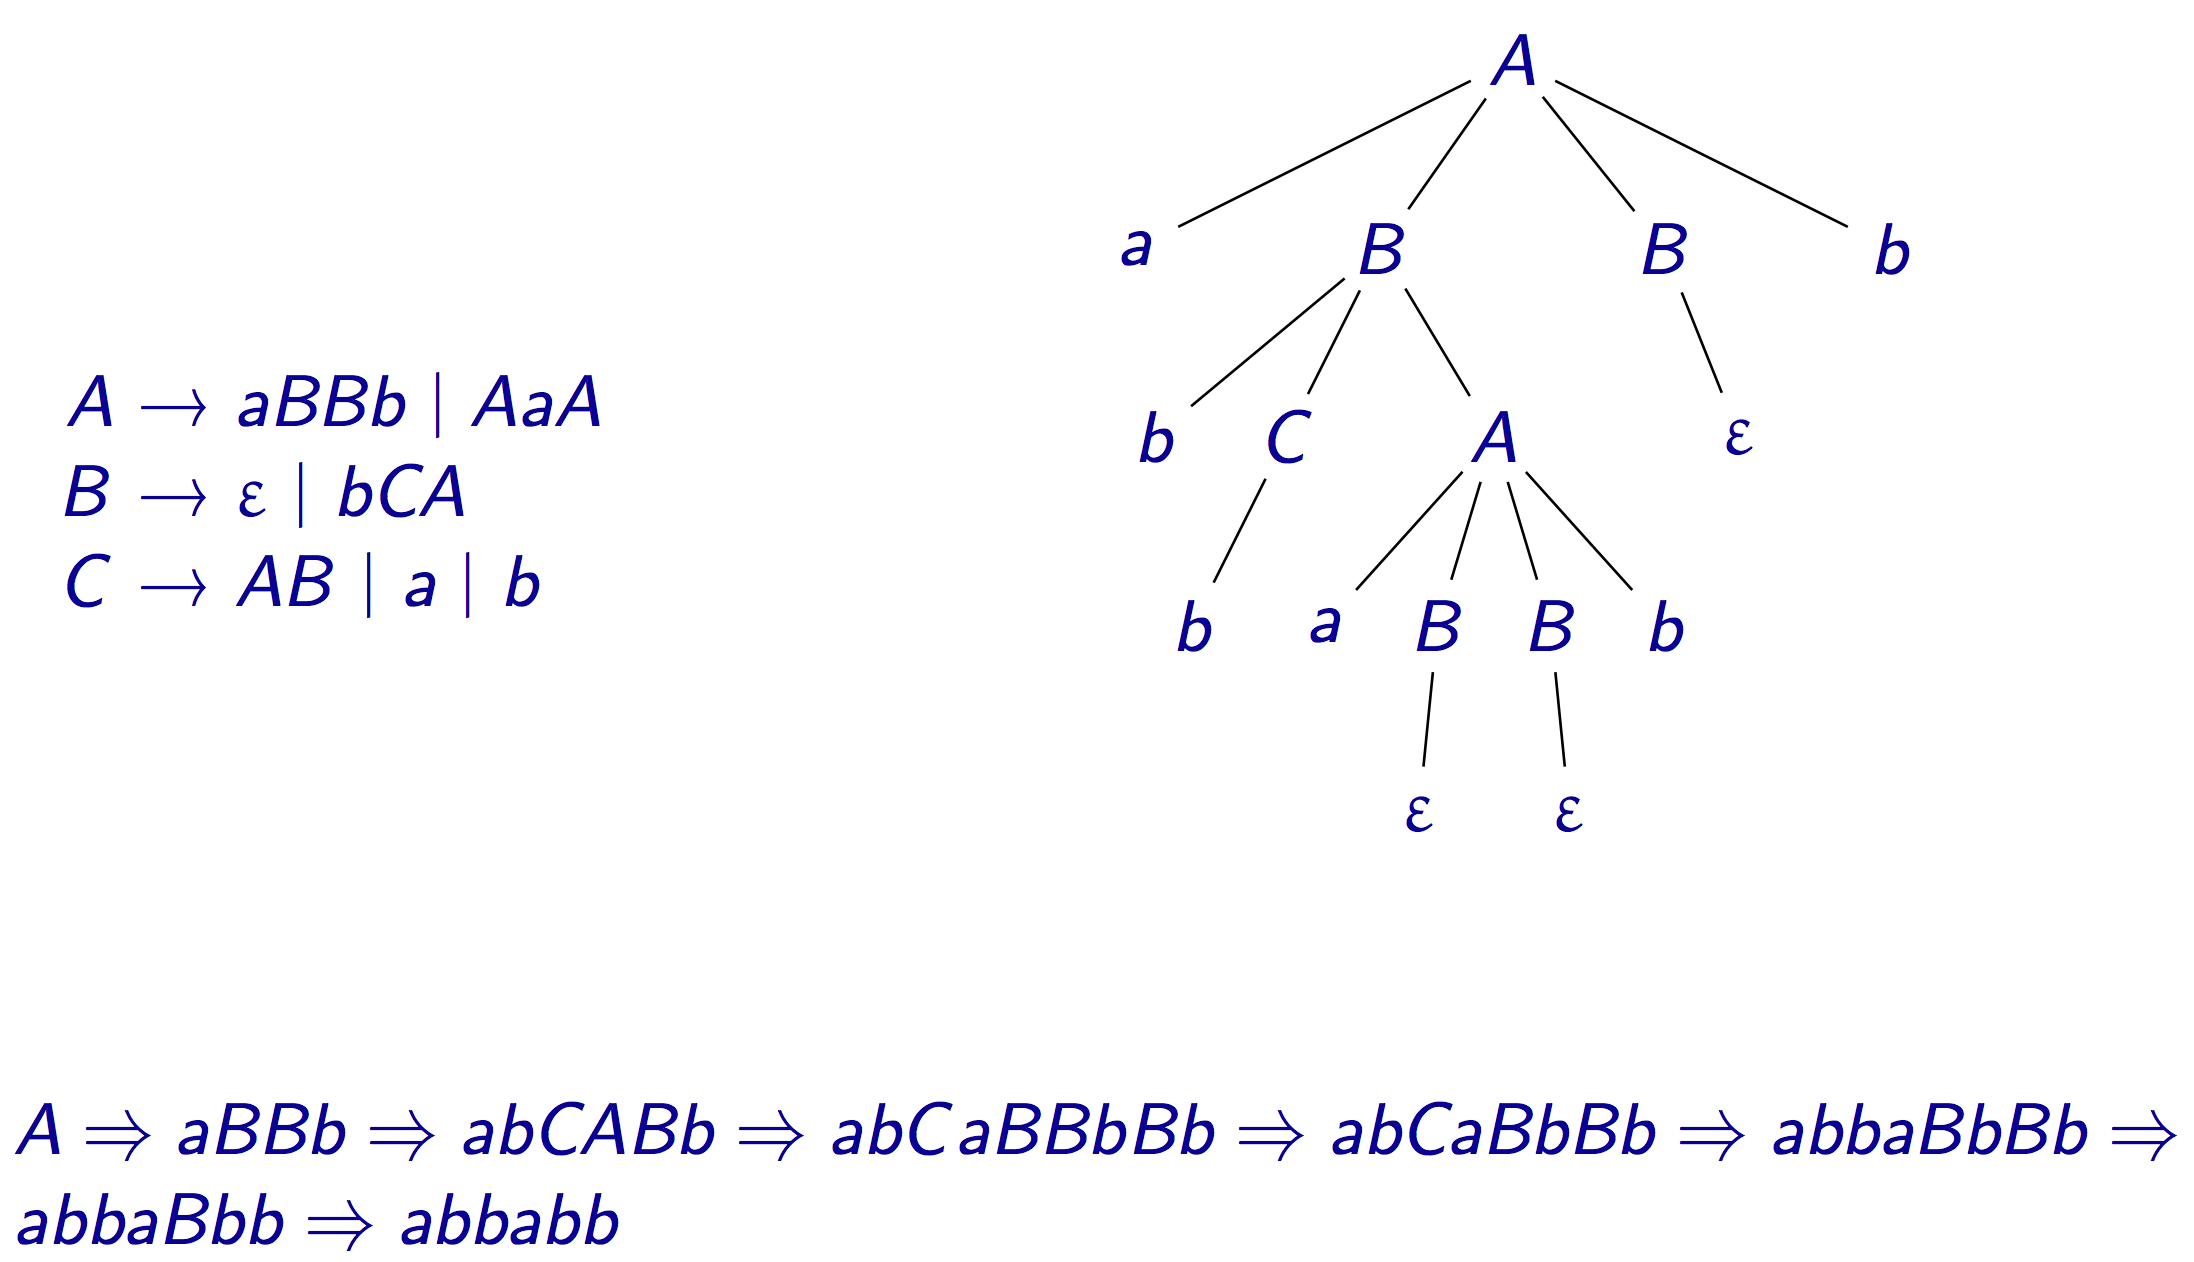
\includegraphics[width=0.6\textwidth]{assets/bg}
\end{figure}

\subsection{Zásobníkové automaty (ZA)}
Slouží k \textbf{rozpoznání bezkontextových jazyků}. S využitím zásobníků si může pamatovat kolik a jaké znaky přečetl, což je potřeba právě k rozpoznání bezkontextového jazyka. Zásobníkový automat je v podstatě konečný automat rozšířený o zásobník. 

\begin{figure}[H]
	\centering
	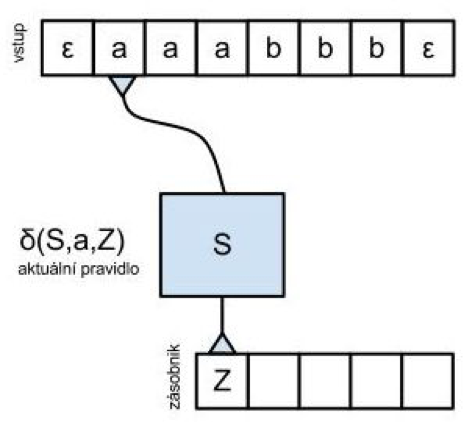
\includegraphics[width=0.30\textwidth]{assets/za}
\end{figure}

\begin{itemize}
\item ZA na základě \textbf{aktuálního znaku} na pásce, \textbf{prvního znaku v zásobníku} a \textbf{aktuálního stavu} změní svůj stav a \textbf{přepíše} znak v zásobníku podle daných pravidel.
\item ZA \textbf{přijímá} dané slovo, jestliže skončí v konfiguraci $(q, \epsilon, \epsilon)$, tedy když se přečte celé vstupní slovo a zásobník je \textbf{prázdný}.
\item \textbf{Konfigurace} je dána: aktuálním stavem, obsahem pásky a obsahem zásobníku.
\item \textbf{Deterministický} -- nesmí se objevit \textbf{stejná konfigurace vícekrát}.
\end{itemize}

\subsubsection{Formální definice zásobníkového automatu}
Zásobníkový automat $M$ je definován jako šestice $M = (Q, \Sigma, \Gamma, \delta, q_0, Z_0)$, kde:
\begin{itemize}
\item $Q$ je konečná neprázdná množina \textbf{stavů}.
\item $\Sigma$ je konečná neprázdná množina \textbf{vstupních symbolů} (vstupní abeceda).
\item $\Gamma$ (\textit{velká gamma}) je konečná neprázdná množina \textbf{zásobníkových symbolů}.
\item $\delta$ je \textbf{přechodová funkce} (konečná množina instrukcí), $\delta: Q \times (\Sigma \cup {\epsilon}) \times \Gamma → P_{\rm fin}(Q \times \Gamma^*)$.
\item $q_0$ je \textbf{počáteční stav}, $q_0 \in Q$.
\item $Z_0$ je \textbf{počáteční zásobníkový symbol}, $Z_0 \in \Gamma$.
\end{itemize}

\subsubsection{Definice instrukcí (pravidel) v ZA}
Instrukce (sady instrukcí reprezentují přechodovou funkci $\delta$) definují \textbf{chování automatu}:
\begin{equation}
(q, a, X) \rightarrow (q', \alpha)\textrm{, kde } a\in \Sigma.
\end{equation}
Tato instrukce je aplikovatelná jen v situaci (neboli konfiguraci), kdy \textbf{řídicí jednotka} je ve stavu $q$, \textbf{čtecí hlava} na vstupní pásce čte symbol $a$ a na vrcholu zásobníku je symbol $X$. Pokud je \textbf{instrukce aplikována}, vykoná se následující:
\begin{enumerate}
\item řídicí jednotka \textbf{přejde do stavu} $q$,
\item čtecí hlava na vstupní pásce se \textbf{posune o jedno políčko doprava},
\item vrchní symbol v zásobníku se \textbf{odebere} (vymaže),
\item \textbf{na vrchol zásobníku se přidá} řetězec $\alpha$ tak, že jeho nejlevější symbol je aktuálním vrcholem zásobníku.
\end{enumerate}

\begin{table}[H]
	\vspace{-2mm}
	\centering
	\begin{tabular}{|l|l|p{6.5cm}|}
		\hline
		\textbf{Pravidlo} & \textbf{Akce (Z = zásobník)} & \textbf{Význam} \\ \hline
		$ \delta(q_1, a, X) \rightarrow (q_1, YX) $ 	&                 \textbf{přidání} prvku do Z & na začátek zásobníku se vloží $Y$ \\ \hline
		$ \delta(q_1, a, X) \rightarrow (q_1, Y) $	&                  \textbf{přepsání} prvku v Z & první prvek zásobníku se přepíše na $Y$ \\ \hline
		$ \delta(q_1, a, X) \rightarrow (q_1, \epsilon) $	&                  \textbf{smazání} prvku ze Z & první prvek zásobníku se smaže neboli nahradí prázdným slovem $\epsilon$ \\ \hline
		$ \delta(q_1, a, X)\rightarrow(q_2, X) $	&                  \textbf{změna stavu}& stav $ q_1 $ se změní na stav $ q_2 $ \\ \hline
		$\delta(q_1, a, X)\rightarrow\emptyset$	&                  \textbf{pád} automatu & ukončení výpočtu, slovo nebylo přijato \\ \hline
	\end{tabular}
\end{table}

\subsection{Převod BG na zásobníkový automat}
Využívá se tzv. metody shora-dolů, která obsahuje pouze \textbf{1 stav}:
\begin{enumerate}
\item pro všechny \textbf{neterminály} vypíšu pravidla typu: $(q, \epsilon, A) \rightarrow \{(q, B), (q, C)\}$,
\item všechny \textbf{terminály} přepíšu na pravidla typu: $(q, a, a) \rightarrow (q, \epsilon)$.
\end{enumerate}

\subsubsection*{Příklad}
\begin{minipage}[t]{0.35\textwidth}
\textbf{Vstupní gramatika:}\\
$S \rightarrow A | B$\\
$A \rightarrow a$\\
$B \rightarrow (c)$\\\smallskip\\
$\Sigma = \{A, B, S\}$\\
$\Gamma = \{a, c, (, )\}$
\end{minipage}
\begin{minipage}[t]{0.65\textwidth}
\textbf{Instrukce, převedené dle výše uvedených pravidel:}\\
$(Q, \epsilon, S) \rightarrow \{(q, A), (q, B)\}$\\
$(Q, \epsilon, A) \rightarrow (q, a)$\\
$(Q, \epsilon, B) \rightarrow (q, (c))$\\\smallskip\\
$(Q, a, a) \rightarrow (q, \epsilon)$\\
$(Q, (, () \rightarrow (q, \epsilon)$\\
$(Q, c, c) \rightarrow (q, \epsilon)$\\
$(Q, ), )) \rightarrow (q, \epsilon)$\\
\end{minipage}